\documentclass{article}

\usepackage{lipsum}
\usepackage{amsfonts}
\usepackage{amsmath}
\usepackage{amsthm}
\usepackage{graphicx}
\graphicspath{{figures/11_18_21_learning_aggregates/}}
\usepackage{epstopdf}
\ifpdf%
  \DeclareGraphicsExtensions{.eps,.pdf,.png,.jpg}
\else
  \DeclareGraphicsExtensions{.eps}
\fi
\usepackage{amsopn}
\DeclareMathOperator{\diag}{diag}
\usepackage{booktabs}
\usepackage{bbm}
\usepackage{bm}
\usepackage{caption}
\usepackage{subcaption}
\usepackage[utf8]{inputenc}
\usepackage[T1]{fontenc}
\usepackage[margin=1in]{geometry}
\usepackage{hyperref}
\usepackage{algorithm}
\usepackage{algpseudocode}

\newcommand{\norm}[1]{\left\lVert#1\right\rVert}
\newcommand{\normtwo}[1]{\left\lVert#1\right\rVert_2}
\newcommand{\abs}[1]{\left\lvert#1\right\rvert}
\newcommand{\mat}[1]{\bm{{#1}}}
\renewcommand{\vec}[1]{\bm{{#1}}}
\newcommand{\lequiv}{\Leftrightarrow}
\newcommand{\bigO}[1]{\mathcal{O}\!\left(#1\right)}
\newcommand{\ceil}[1]{\left\lceil #1 \right\rceil}
\newcommand{\floor}[1]{\left\lfloor #1 \right\rfloor}
\newcommand{\sfrac}[2]{#1/#2}
\newcommand{\hquad}{\enskip}
\newcommand{\expected}[1]{\mathbb{E}\left[#1\right]}
\newcommand{\mspan}[1]{\text{span}\left( #1 \right)}
\newcommand{\prob}[1]{P\left(#1\right)}
\newcommand{\probt}[1]{P\left( \text{#1} \right)}
\newcommand{\condprob}[2]{P\left(#1 \:|\: #2\right)}
\newcommand{\condprobt}[2]{P\left(\text{#1} \:|\: \text{#2}\right)}
\newcommand{\bayes}[2]{\frac{\condprob{#2}{#1}\prob{#1}}{\prob{#2}}}
\newcommand{\bayesx}[3]{\frac{\condprob{#2}{#1}\prob{#1}}{\condprob{#2}{#1}\prob{#1} + \condprob{#2}{#3}\prob{#3}}}
\newcommand{\sech}{\text{sech}}
\newcommand*{\vertbar}{\rule[-1ex]{0.5pt}{2.5ex}}
\newcommand*{\horzbar}{\rule[.5ex]{2.5ex}{0.5pt}}
\newcommand{\vect}[2]{\underline{{#1}}_{{#2}}}
\newcommand{\basisp}[1]{\underline{{p}}_{{#1}}}
\newcommand{\basisq}[1]{\underline{{q}}_{{#1}}}
\newcommand{\coeff}[1]{\underline{{a}}_{{#1}}}
\newcommand{\bestfit}{\underline{\bar{x}}}
\newcommand{\grad}{\nabla}
\newcommand{\laplace}{\Delta}
\newcommand{\setbar}{\:\middle|\:}
\renewcommand{\div}{\grad \cdot}
\renewcommand{\Re}{\text{Re}}

\begin{document}
\section{Background}
Here, we are attempting to train an ML agent to output both aggregates and interpolation for an AMG solver given some matrix $\mat{A}$.  We will be exploring 4 test problems:
\begin{enumerate}
\item 1D Poisson with Dirichlet conditions
\item 1D Poisson with Neumann conditions
\item 2D isotropic Poisson with Dirichlet conditions
\item 2D rotated anisotropic Poisson with Dirichlet conditions.  This problem is rotated by $\theta=\frac{\pi}{6}$ and with a scaling of $0.001$ in the $y$-direction.
\end{enumerate}

\section{Aggregation and Interpolation Algorithm}
To compute the aggregates and final interpolation operator, two individual networks are trained concurrently to perform each action, which we will label $\Theta_{\text{Agg}}$ and $\Theta_{\text{Interp}}$, both taking some weighted graph and returning a new graph with same connectivity, but different weight values.  The algorithm for finding the aggregates and interpolation is roughly sketched below:
\begin{enumerate}
\item Let $\mat{A} \in \mathbb{R}^{n \times n}$ be the system we are trying to solve and $\alpha \in \left(0, 1\right]$ be some parameter that determines the ratio of aggregates to vertices, i.e. we will be roughly coarsening the graph by $1/\alpha$.  Define $k := \ceil{\alpha n}$, the number of aggregates we will be outputting.
\item Convolve the graph of $\mat{A}$ with $\Theta_{\text{Agg}}$ to obtain a new set of node values and edge values.  We will use the node values as a \textit{scoring} and the edge values as path weights.  Define the aggregate centers as the indices of the largest $k$ node scores.  Then, run Bellman-Ford on the graph with these aggregate centers and new edge weights to obtain a tentative aggregation operator, $\text{Agg}$.
\item Now, again convolve the graph of $\mat{A}$ but with $\Theta_{\text{Interp}}$ (with aggregate information) to obtain the aggregate smoother $\mat{\hat{P}}$.  Form $\mat{P} := \mat{\hat{P}}\text{Agg}$.
\end{enumerate}

\section{Genetic Training}
Training of both networks is done at the same time with PyGAD\cite{gad2021pygad}, a genetic algorithm that can be used to train networks without any gradient information.  A basic overview of the training algorithm is that the method is seeded with some number of randomly generated networks. A subset of the best performing (most fit) networks are selected and ``bred'' with one another (crossing weights/traits) and ``mutations'' inserted (random perturbations to weights) to create another population of networks.  This is then repeated for many ``generations'' until a set of hopefully trained networks is obtained, from which we can pick the best fit as our final network.

\section{Results}
Results for selecting aggregates and interpolation are visualized in figures \ref{fig:1d_dirichlet} - \ref{fig:2d_anisotropic}.  Aggregates are visualized as colored blobs, aggregate centers are $\star$s, and edge weights for Bellman Ford are shown mapped from dark coloring (low weight) to vivid colors (high weight).

\begin{figure}[b]
  \centering
  \begin{subfigure}[b]{\textwidth}
    \centering
    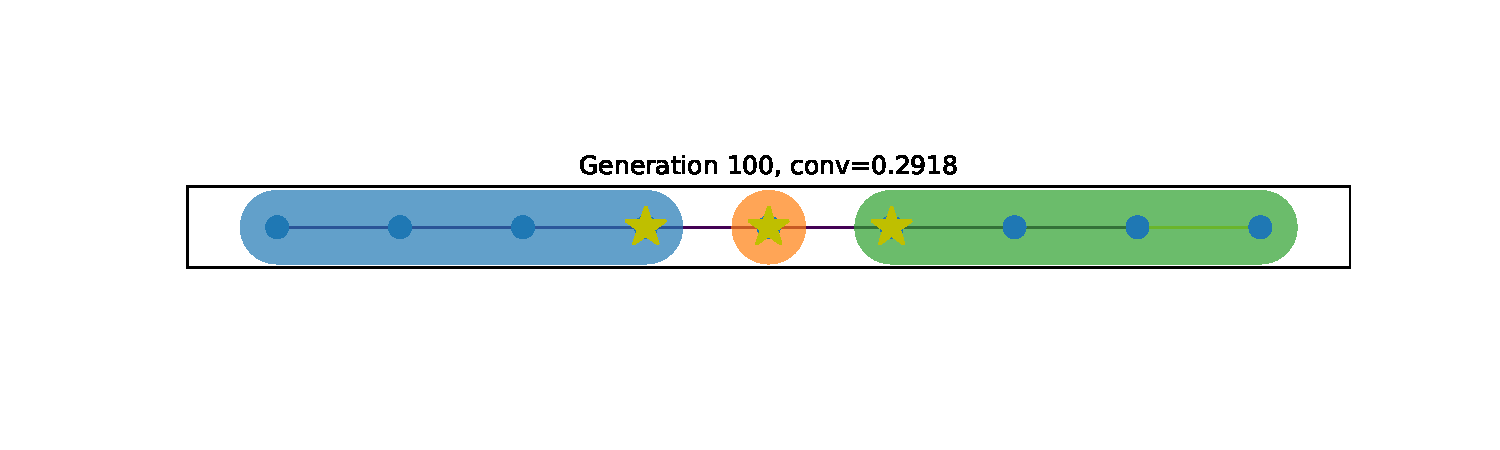
\includegraphics[width=\textwidth, trim=0 80 0 70, clip]{1d_dirichlet_figures/100_agg.pdf}
    \caption{ML Aggregates}
  \end{subfigure}
  \hfill
  \begin{subfigure}[b]{\textwidth}
    \centering
    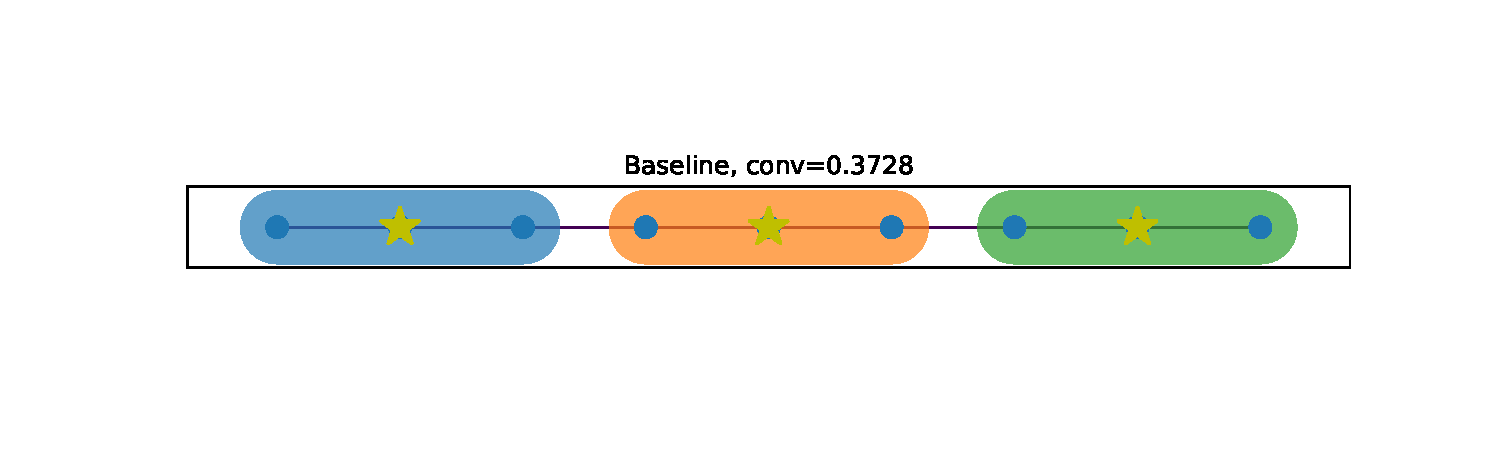
\includegraphics[width=\textwidth, trim=0 80 0 70, clip]{1d_dirichlet_figures/baseline.pdf}
    \caption{Baseline Aggregates (coarsening by 3)}
  \end{subfigure}
  \caption{Aggregates for 1D Dirichlet problem}
  \label{fig:1d_dirichlet}
\end{figure}

\begin{figure}[b]
  \centering
  \begin{subfigure}[b]{\textwidth}
    \centering
    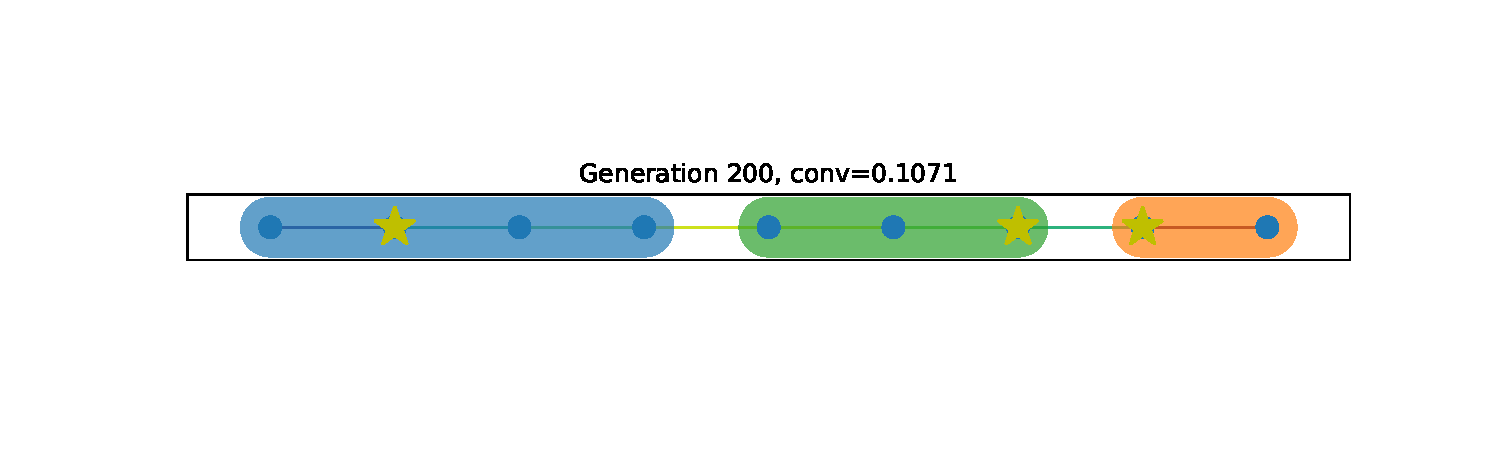
\includegraphics[width=\textwidth, trim=0 90 0 70, clip]{1d_neumann_figures/200_agg.pdf}
    \caption{ML Aggregates}
  \end{subfigure}
  \hfill
  \begin{subfigure}[b]{\textwidth}
    \centering
    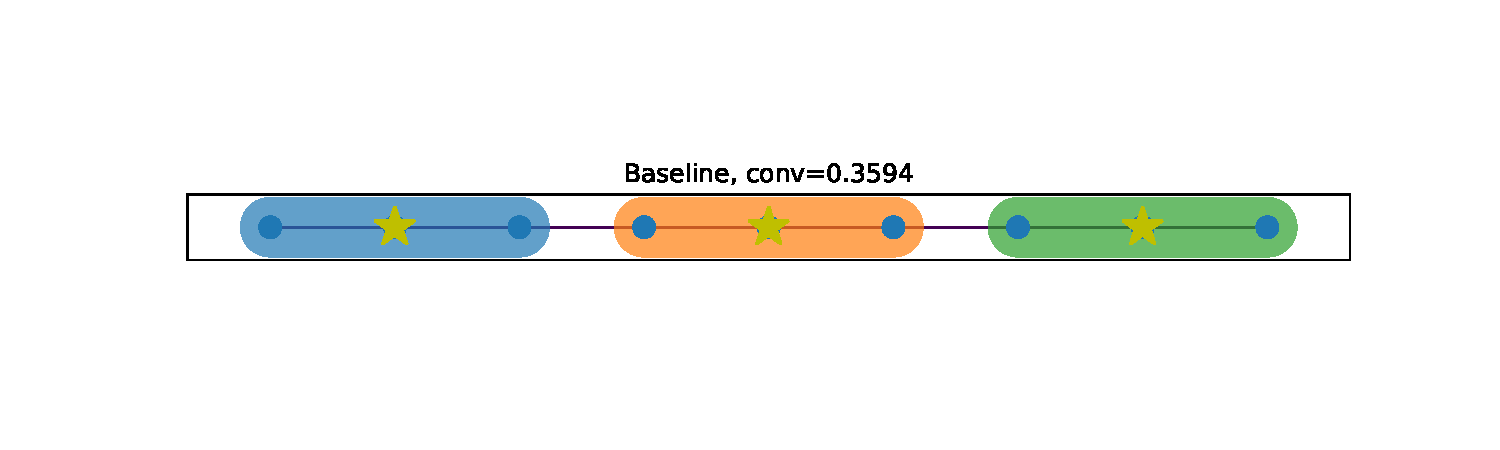
\includegraphics[width=\textwidth, trim=0 90 0 70, clip]{1d_neumann_figures/baseline.pdf}
    \caption{Baseline Aggregates (coarsening by 3)}
  \end{subfigure}
  \caption{Aggregates for 1D Neumann problem}
  \label{fig:1d_neumann}
\end{figure}

\begin{figure}[b]
  \centering
  \begin{subfigure}[b]{0.8\textwidth}
    \centering
    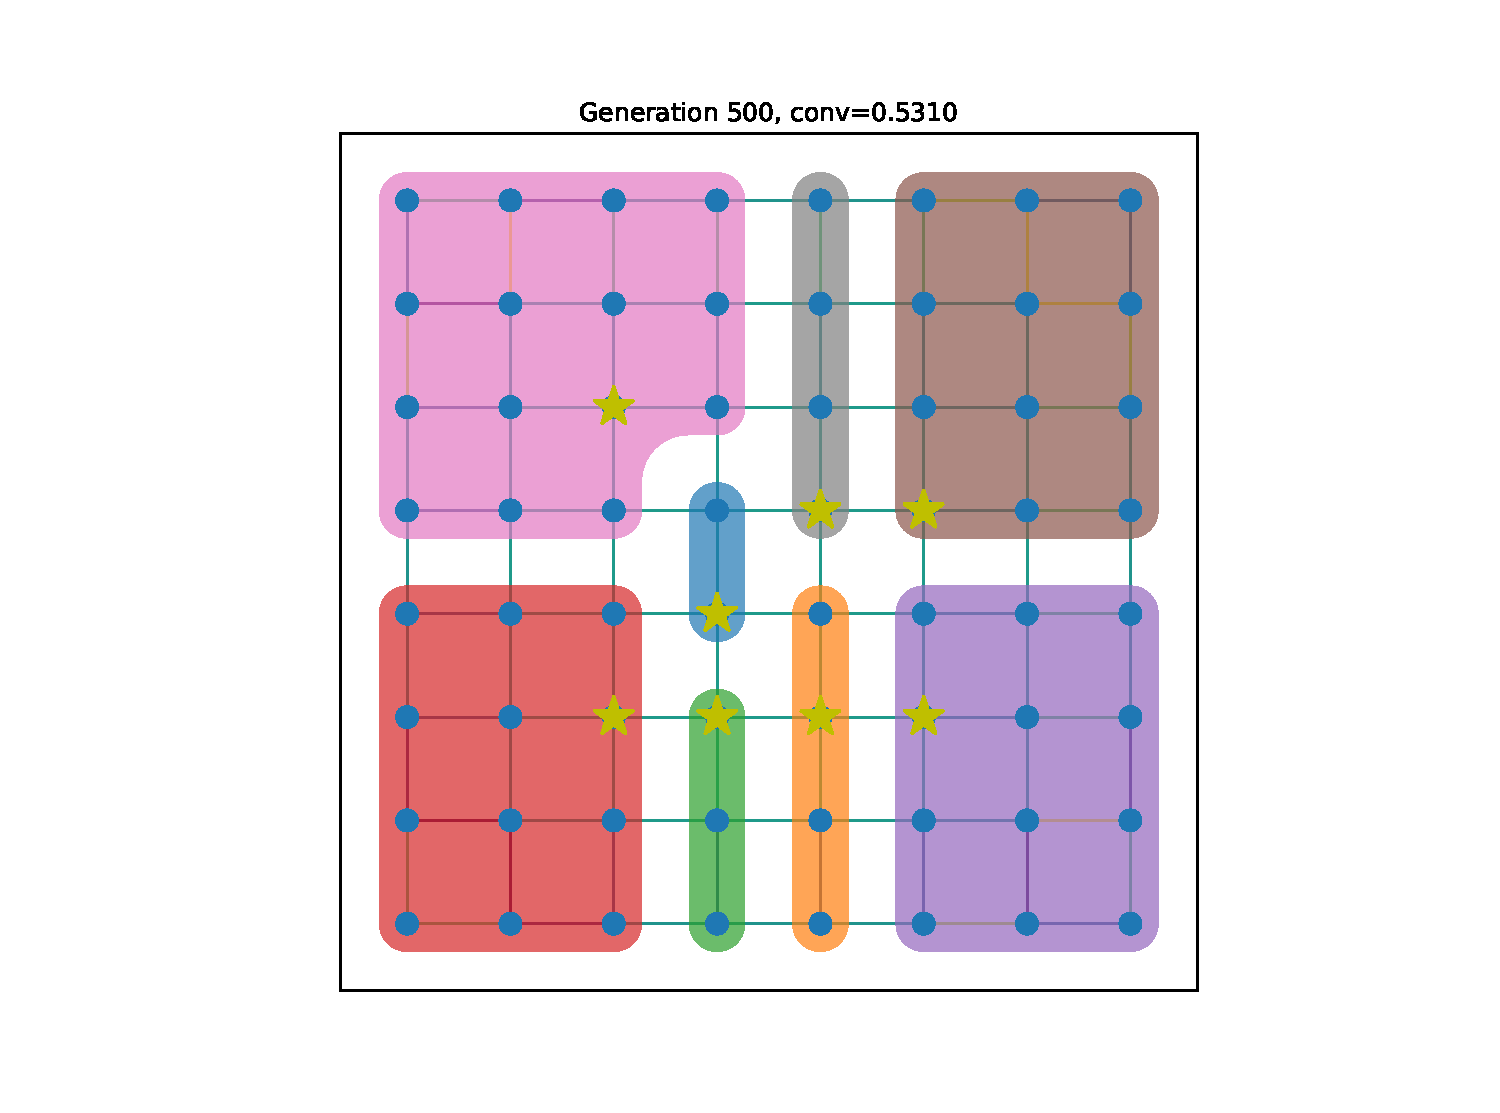
\includegraphics[height=4in, trim=100 0 100 0, clip]{2d_isotropic_figures/500_agg.pdf}
    \caption{ML Aggregates}
  \end{subfigure}
  \hfill
  \begin{subfigure}[b]{0.8\textwidth}
    \centering
    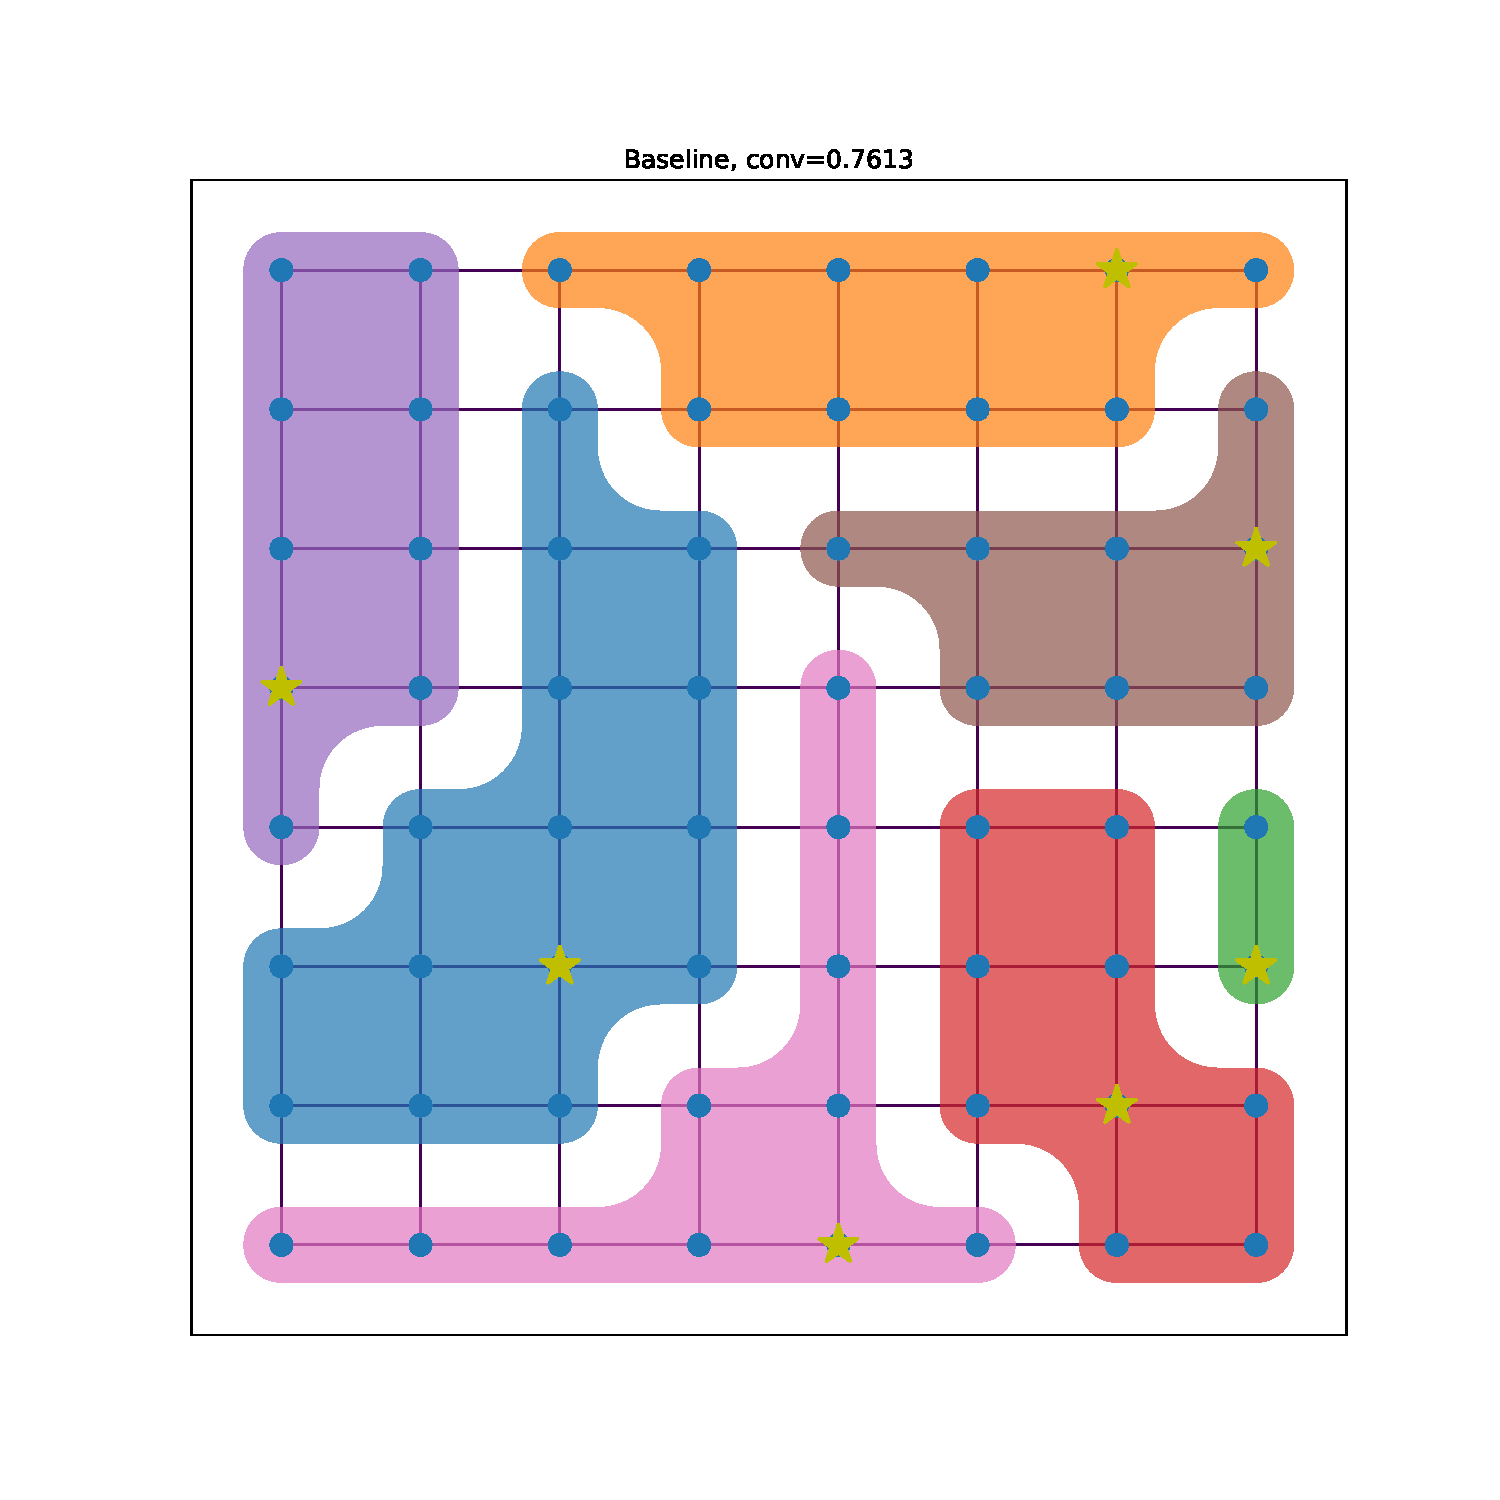
\includegraphics[height=4in]{2d_isotropic_figures/baseline.pdf}
    \caption{Lloyd Aggregates}
  \end{subfigure}
  \caption{Aggregates for isotropic 2D Poisson}
  \label{fig:2d_isotropic}
\end{figure}

\begin{figure}[b]
  \centering
  \begin{subfigure}[b]{0.6\textwidth}
    \centering
    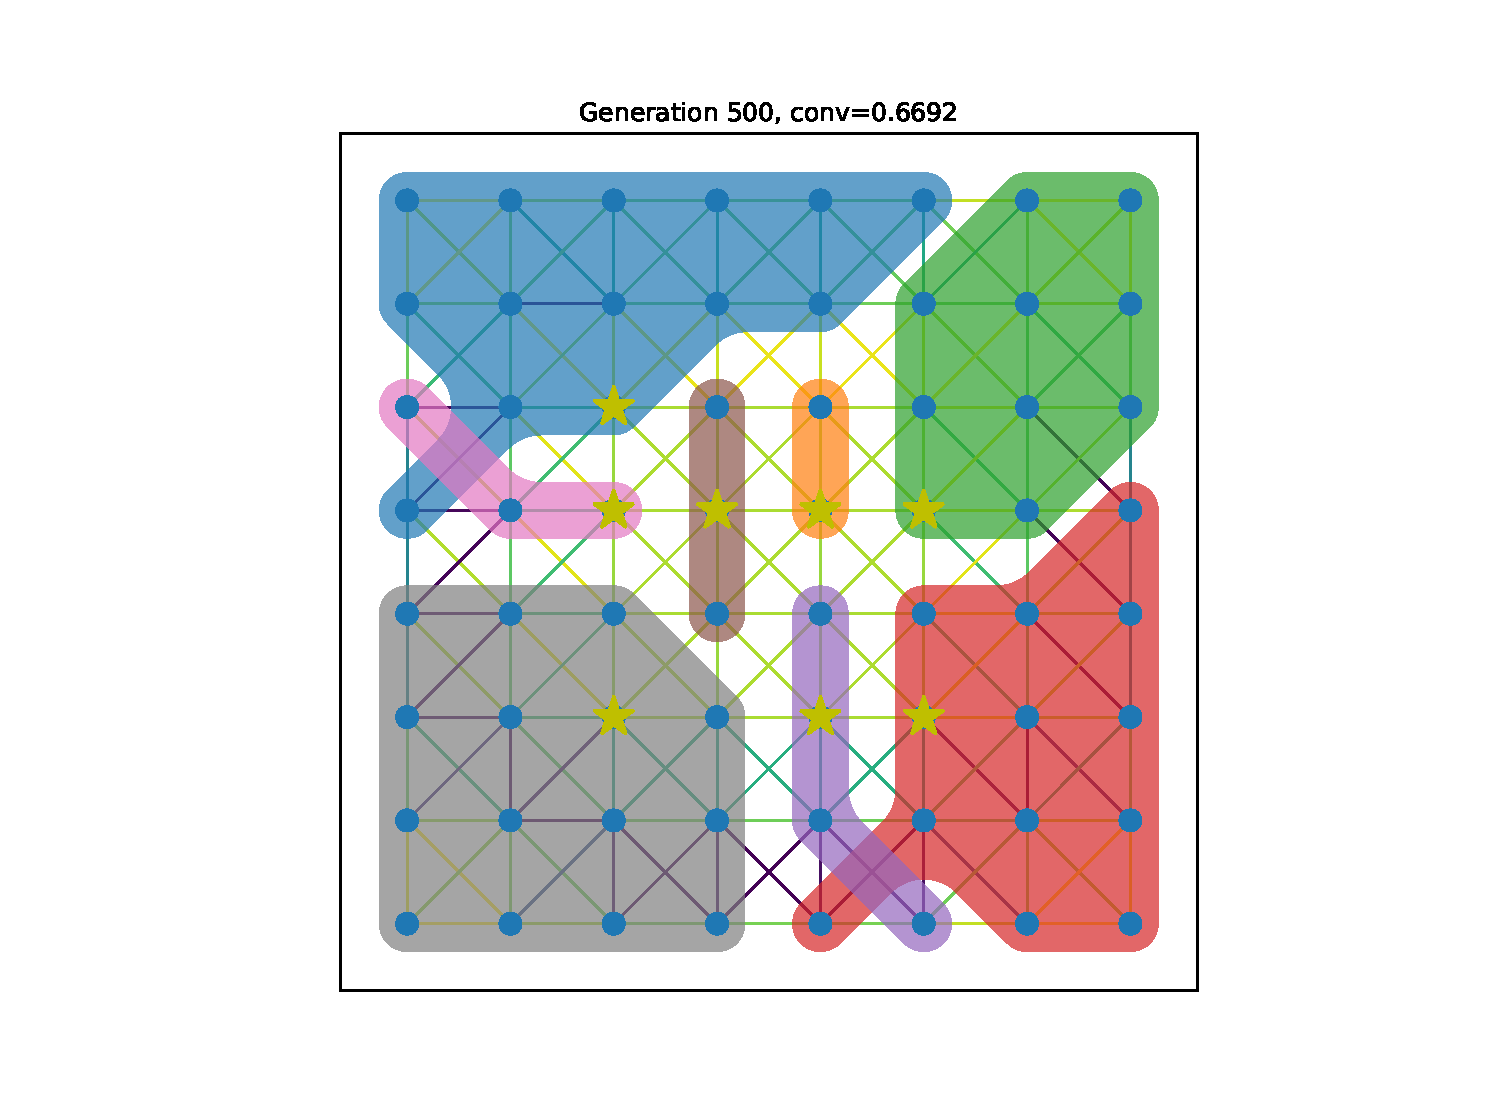
\includegraphics[height=4in, trim=100 0 100 0, clip]{2d_anisotropic_figures/500_agg.pdf}
    \caption{ML Aggregates}
  \end{subfigure}
  \hfill
  \begin{subfigure}[b]{0.6\textwidth}
    \centering
    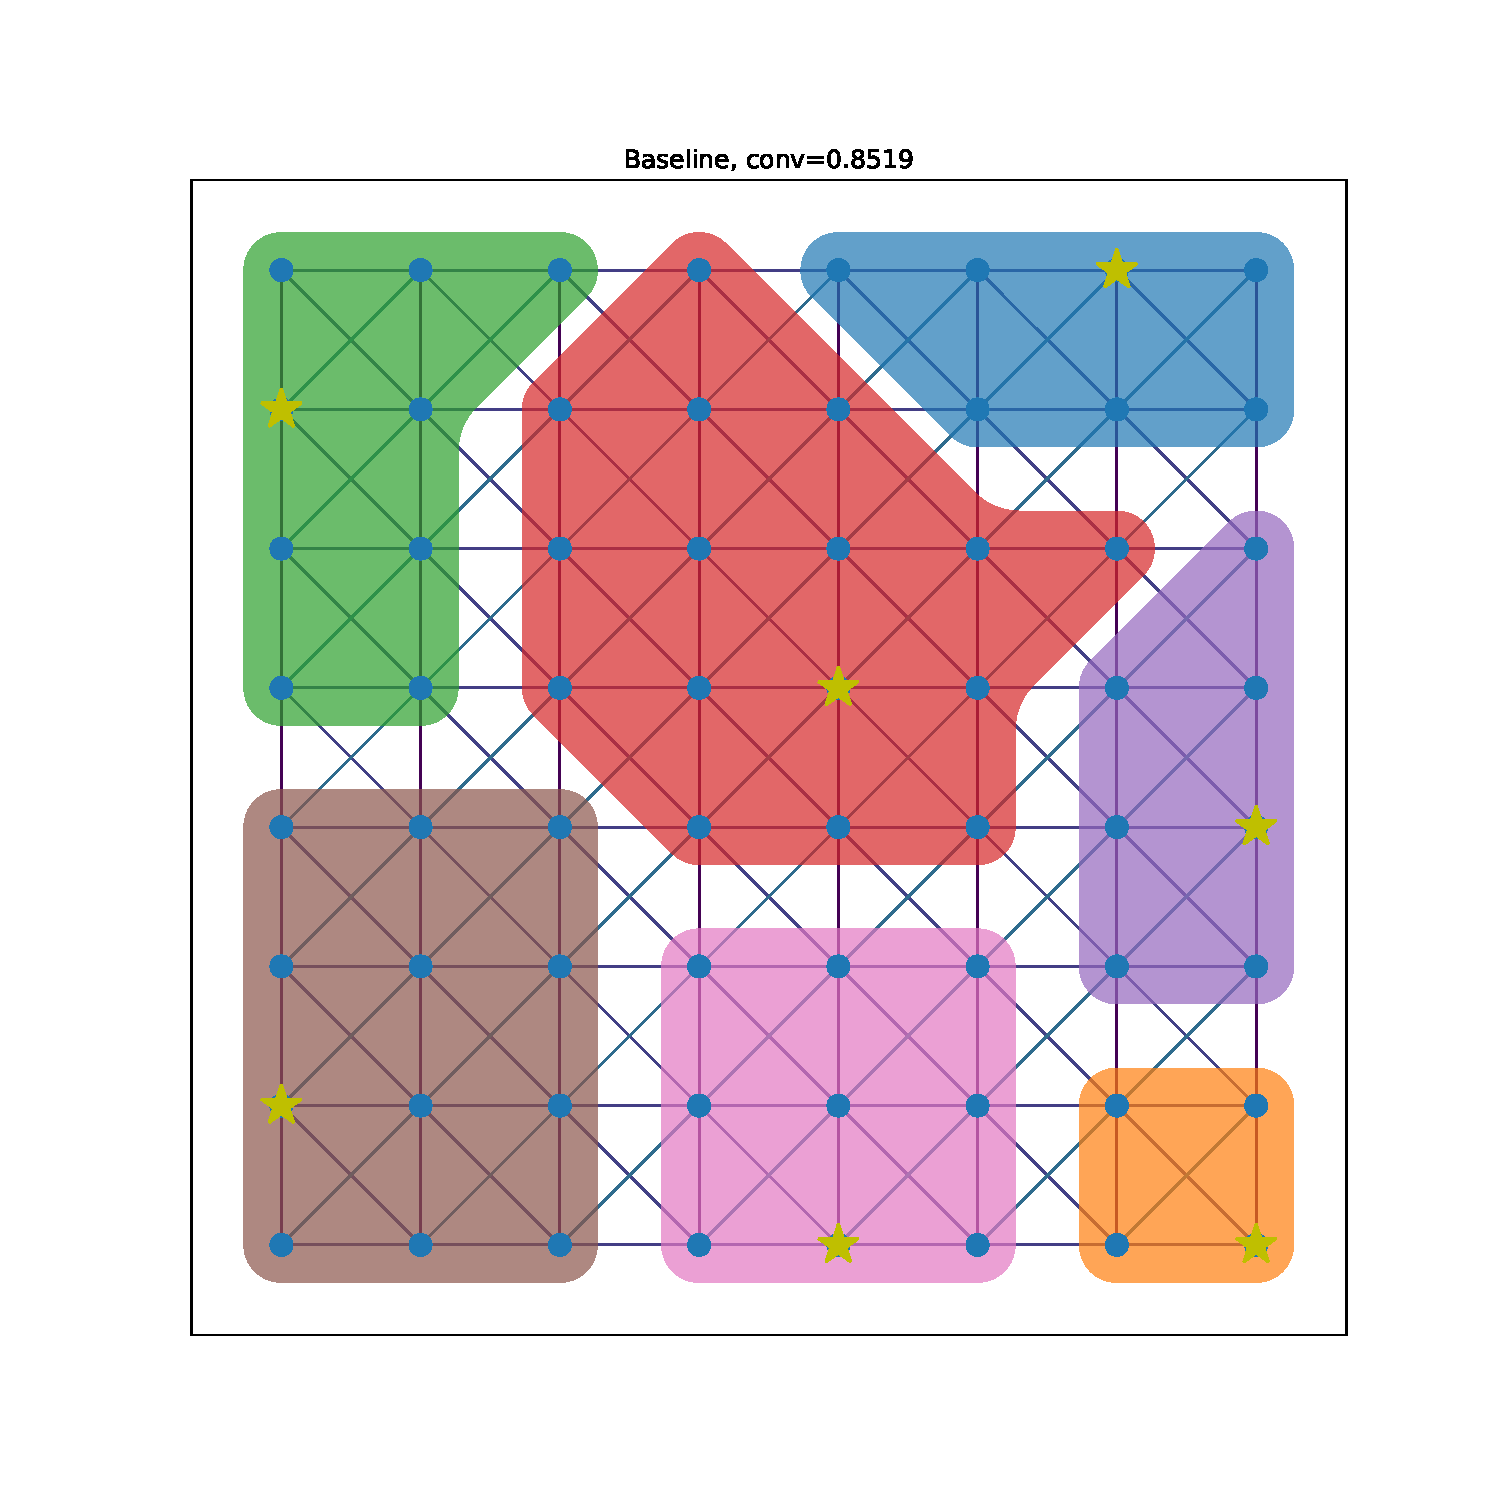
\includegraphics[height=4in]{2d_anisotropic_figures/baseline.pdf}
    \caption{Lloyd Aggregates}
  \end{subfigure}
  \caption{Aggregates for anisotropic 2D Poisson}
  \label{fig:2d_anisotropic}
\end{figure}

\section{Future}
Perhaps an obvious future direction to explore is to perform an ablation study, comparing results for the following cases:
\begin{enumerate}
\item Lloyd aggregation and SA interpolation (baseline)
\item ML Aggregation and SA interpolation
\item Lloyd aggregation and ML interpolation (somewhat what was done before)
\item ML Aggregation and interpolation trained together (results from above)
\item ML Aggregation and interpolation trained separately, then combined
\end{enumerate}

Also, it would likely be worth exploring use of the GA vs. traditional gradient based optimizers.  The results above suggest that the GA is able to broadly learn effective networks, and the algorithm was able to effectively learn an interpolation for the 1D Neumann case where previously the gradient optimizer could not.  Perhaps a hybrid approach could be employed where the network is first broadly trained with the genetic algorithm then refined with gradient descent.

\bibliographystyle{siam}
\bibliography{navier}
\end{document}
